\documentclass{Interspeech}

% 2023-10-21 modified by Simon King (Simon.King@ed.ac.uk)  
% 2024-01 modified by TPC Chairs of Interspeech 2024  
% 2024-10 modified by Antoine Serrurier for Interspeech 2025
% 2024-12 modified by TPC Chairs of Interspeech 2025

% **************************************
% *    DOUBLE-BLIND REVIEW SETTINGS    *
% **************************************
% Comment out \interspeechcameraready when submitting the 
% paper for review.
% If your paper is accepted, uncomment this to produce the
%  'camera ready' version to submit for publication.

\interspeechcameraready 


% **************************************
% *                                    *
% *      STOP !   DO NOT DELETE !      *
% *          READ THIS FIRST           *
% *                                    *
% * This template also includes        *
% * important INSTRUCTIONS that you    *
% * must follow when preparing your    *
% * paper. Read it BEFORE replacing    *
% * the content with your own work.    *
% **************************************

% title here must exactly match the title entered into the paper submission system
\title{Evaluating Logit-Based GOP Scores for Mispronunciation Detection}

% the order of authors here must exactly match the order entered into the paper submission system
% note that the COMPLETE list of authors MUST be entered into the paper submission system at the outset, including when submitting your manuscript for double-blind review
\author{Aditya Kamlesh}{Parikh}
\author{Cristian}{Tejedor-Garcia}
\author{Catia}{Cucchiarini}
\author{Helmer}{Strik}

%The maximum number of authors in the author list is 20. If the number of contributing authors is more than this, they should be listed in a footnote or the acknowledgement section.

% if you have too many addresses to fit within the available space, try removing the "\\" newlines
\affiliation[nocounter]{Centre for Language Studies}{Radboud University}{the Netherlands}
\email{aditya.parikh@ru.nl, cristian.tejedorgarcia@ru.nl, catia.cucchiarini@ru.nl, helmer.strik@ru.nl}
\keywords{GOP, logit-based GOP, mispronunciation detection, pronunciation assessment,  softmax posterior probabilities}

\newcommand{\blue}[1]{\textcolor{blue}{#1}}
\usepackage{comment}
\usepackage{graphicx}

\usepackage{tabularx}
\usepackage{booktabs}
\usepackage{multirow}
\usepackage{subfig}
\usepackage{comment}
\usepackage[utf8]{inputenc} % Enables UTF-8 encoding
\usepackage{graphicx} % Optional, if you plan to include graphics
\usepackage{amsmath} % For math symbols
\usepackage{amssymb} % For special symbols
\usepackage{array} % For better table alignment
\usepackage{enumitem} 
\usepackage{tipa} 
\usepackage{booktabs}



\begin{document}

\maketitle

% the abstract here must exactly match the abstract entered into the paper submission system 
%1000 ASCII char max
\begin{abstract}
Pronunciation assessment relies on goodness of pronunciation (GOP) scores, traditionally derived from softmax-based posterior probabilities. However, posterior probabilities may suffer from overconfidence and poor phoneme separation, limiting their effectiveness. This study compares logit-based GOP scores with probability-based GOP scores for mispronunciation detection. We conducted our experiment on two L2 English speech datasets spoken by Dutch and Mandarin speakers, assessing classification performance and correlation with human ratings. Logit-based methods outperform probability-based GOP in classification, but their effectiveness depends on dataset characteristics. The maximum logit GOP shows the strongest alignment with human perception, while a combination of different GOP scores balances probability and logit features. The findings suggest that hybrid GOP methods incorporating uncertainty modeling and phoneme-specific weighting improve pronunciation assessment.
\end{abstract}




\section{Introduction}
\label{sec:Introduction}


In today's interconnected world, globalization has led to increased movement across borders for work, education, and other opportunities. For individuals who are adapting to a new linguistic environment, learning the local language is essential for social integration, career advancement, and overall well-being \cite{kuschel2023combining}. Effective communication goes beyond knowing the vocabulary and grammar: A clear pronunciation is equally important, as it impacts intelligibility, confidence, and the ability to engage in meaningful conversations \cite{reading101017,jenkins2000phonology}. Poor pronunciation can lead to misunderstandings, impede effective social interactions and even create barriers in academic and professional settings \cite{zossadult}. However, mastering pronunciation in a second language (L2) can be challenging. Differences between the first language (L1) and the target language often result in persistent pronunciation errors. These difficulties are further compounded by the limited tools and resources available to language instructors for providing personalized pronunciation feedback.

To address these challenges, Computer-Assisted Pronunciation Training (CAPT) systems have gained popularity \cite{hsu2024examination,Amrate2024ComputerassistedPT}. A key component of these systems is Mispronunciation Detection and Diagnosis (MDD), which helps learners identify and correct pronunciation errors in real time \cite{alrashoudi2025improving}. Phoneme-level assessment, in particular, provides more precise feedback than broader word- or sentence-level evaluations, allowing learners to focus on specific areas for improvement \cite{cao2024framework}. One of the most widely used methods for detecting phoneme-level mispronunciations is the goodness of pronunciation (GOP) score \cite{witt2000use}.


GOP was initially introduced as a measure of pronunciation quality, estimating the probability of a phoneme and comparing it against a predefined threshold to flag mispronunciations \cite{kanters2009goodness}. Over time, several enhancements have improved its accuracy. Weighted-GOP \cite{doremalen10_interspeech} adjusts phoneme scores based on linguistic and acoustic factors, prioritizing phonemes prone to mispronunciation. Lattice-based GOP \cite{5451809} considers multiple pronunciation possibilities using phoneme lattices, yielding more robust confidence scores. Context-aware GOP \cite{shi2020context} incorporates phoneme transitions and durations to better capture natural pronunciation variations. More recently, multidimensional GOP features \cite{do2024acoustic,cao2024framework,gong_gopt} have been introduced, leveraging richer feature representations beyond simple probability thresholds for more precise mispronunciation detection. 

Despite these advancements, GOP methods face challenges in data availability and computational efficiency \cite{elkheir2023mispronunciation}. Annotated pronunciation data, including prosody and fluency scores, requires expert evaluation, making large-scale collection expensive. Additionally, traditional GOP methods scale poorly with phoneme size because of an increasing number of features and increasing computational costs. This highlights the need for a fast, robust, and non-trainable GOP computation method.

More recently, foundation models \cite{babu2021xls,10.1109/TASLP.2021.3122291} trained on massive amounts of data have been used to improve MDD. These models can be fine-tuned with significantly less data, addressing some of the data availability constraints faced by traditional GOP-based methods. GOP scores can be derived from a forced alignment using Connectionist Temporal Classification (CTC)-based phoneme recognition models, which rely on posterior probabilities generated by acoustic models. These probabilities are obtained through softmax normalization of model logits, which is a widely adopted method \cite{sudhakara2019improved}. However, softmax-based probability estimates suffer from overconfidence \cite{pearce2021understanding,wei2022mitigating}, inflating confidence in incorrect phoneme predictions and reducing the granularity needed to detect subtle mispronunciations. This issue is particularly problematic in phoneme recognition for children's speech and non-native speakers, where articulatory deviations are very common \cite{xie2020comparing,preston2015perception}.

To address these limitations, we propose a logit-based GOP method that directly utilizes raw logits from CTC-based models rather than softmax-normalized probabilities. Logits retain more discriminative information and avoid the gradient saturation problem inherent in softmax-based scoring \cite{li2020learning}. We explore four logit-based metrics to enhance mispronunciation detection: Maximum Logit (GOP\textsubscript{MaxLogit}), Mean Logit Margin \cite{10147340} (GOP\textsubscript{Margin}), Logit Variance (GOP\textsubscript{LogitVariance}), and combined (hybrid) logit-probability GOP\textsubscript{Combined} scores. This novel approach provides a fast, robust, and non-trainable solution, crucial for real-time phoneme assessment.

Our method builds upon prior work on uncertainty quantification in pronunciation assessment, such as \cite{yeo2023speech}, which applies GOP-based scores to dysarthric speech. However, prior studies have not explicitly investigated the use of raw logits in GOP calculations. Our approach fills this gap by utilizing logit-based metrics to improve accuracy and reliability in pronunciation assessment.
%This highlights the need for a fast, robust, and non-trainable method to compute GOP. When using GOP scores based on forced alignment with a CTC-based phoneme recognition model, traditional GOP methods derive scores from posterior probabilities generated by acoustic models. These approaches typically compute GOP using the negative log of phoneme-specific posterior probabilities, obtained through softmax normalization of model logits—a widely adopted method \cite{sudhakara2019improved}. However, a critical limitation of this approach lies in the inherent weaknesses of softmax-based probability estimates, which compromise the reliability and discriminative power of GOP scores. This is mainly because of softmax overconfidence \cite{pearce2021understanding,wei2022mitigating}. Building upon this, the overconfidence in softmax probabilities leads to inflated confidence in incorrect phoneme predictions, reducing the granularity needed to detect subtle mispronunciations. This is particularly problematic for phoneme recognition tasks, where slight articulatory deviations are common when it comes to children speech or non-native speakers \cite{xie2020comparing,preston2015perception}. To address this issue, we propose an alternative approach that utilize the raw logits from the CTC-based model rather than the softmax-normalized probabilities. Logits retain more discriminative information and avoid the gradient saturation problem inherent in softmax \cite{li2020learning}. By focusing on logit-based metrics such as Maximum Logit, Mean Logit Margin, and Logit Variance and combined logit-probability score we can achieve more accurate and reliable GOP scores that better capture the nuances of mispronunciations. This method offers a fast, robust, and non-trainable solution, which is crucial for real-time phoneme assessment. This logit-based approach builds upon prior work, such as \cite{yeo2023speech}, which explores various uncertainty quantification techniques for dysarthric speech using a GOP-based framework. However, their study does not explicitly investigate the use of raw logits in GOP calculations or analyze its implications. Our approach fills this gap by using logit-based metrics to enhance the accuracy and reliability of pronunciation assessment.
Our leading research question (RQ) is: To what extent does a logit-based GOP score enhance mispronunciation detection and improve correlation with human rater scores compared to traditional softmax-based GOP scores?


\section{Methodology}
\subsection{Definition of GOP}

The GOP score, first introduced by Witt and Young~\cite{witt2000use}, quantifies pronunciation quality by comparing the likelihood of a hypothesized phoneme to competing alternatives. For a phoneme \( p \) aligned to an audio segment, the original GOP formulation computes:
\begin{equation}
    \text{GOP}_{\text{original}}(p) = \log \frac{P(\mathbf{X} | p)}{ \frac{1}{N} \sum_{q \in \mathcal{Q}} P(\mathbf{X} | q) }
    \label{eq:gop_original}
\end{equation}
where \( P(\mathbf{X} | p) \) is the likelihood of the acoustic features \( \mathbf{X} \) given phoneme \( p \), and \( \mathcal{Q} \) represents competing phonemes.

With deep neural networks (DNNs), GOP is derived from posterior probabilities using the negative log of the mean softmax output over aligned frames \cite{hu2013new}:
\begin{equation}
    \text{GOP}_{\text{DNN}}(p) = -\log \left( \frac{1}{T} \sum_{t=1}^T P(p | \mathbf{x}_t) \right)
    \label{eq:gop_dnn}
\end{equation}
where \( P(p | \mathbf{x}_t) \) is the softmax probability of phoneme \( p \) at frame \( t \) and $T$ is the total number of frames in the phoneme segment.  This equation interprets the mean softmax probability of the target phoneme as a probabilistic measure of pronunciation quality. This approach inherits softmax limitations such as overconfidence and gradient saturation.

\subsection{Logit-Based GOPS}
To address softmax limitations, we propose four novel metrics using raw logits, defined below.

\subsubsection{GOP\textsubscript{MaxLogit}}
This metric captures the model's peak confidence in the target phoneme \( p \) across aligned frames \( t_1 \) to \( t_2 \):
\begin{equation}
    \text{GOP}_{\text{MaxLogit}}(p) = \max_{t \in [t_1, t_2]} \mathbf{l}_t^{(p)}
    \label{eq:gop_maxlogit}
\end{equation}
where \( \mathbf{l}_t^{(p)} \) is the logit for phoneme \( p \) at frame \( t \). It identifies unambiguous articulations but may emphasize transient spikes.

\subsubsection{GOP\textsubscript{Margin}}
This measure quantifies the average superiority of the target phoneme over its strongest competitor. For each frame, we compute the difference (or margin) between the target logit and the highest competing logit. The average of these margins over the segment indicates how well-separated the target phoneme is from other phonemes. This helps in cases where pronunciation errors cause phoneme confusion, which may not always be reflected in probability scores.

\begin{equation}
    \text{GOP}_{\text{Margin}}(p) = \frac{1}{T} \sum_{t=t_1}^{t_2} \left( \mathbf{l}_t^{(p)} - \max_{k \neq p} \mathbf{l}_t^{(k)} \right),
    \label{eq:gop_margin}
\end{equation}


\subsubsection{\texorpdfstring{GOP\textsubscript{VarLogit}}{GOP VarLogit}}

This metric measures the \textit{variability} of the model's confidence in predicting the target phoneme across timeframes. 

\vspace{-0.2cm}
\begin{equation}
    \text{GOP}_{\text{VarLogit}}(p) = \frac{1}{T} \sum_{t=t_1}^{t_2} \left( \mathbf{l}_t^{(p)} - \mu_p \right)^2, \quad \mu_p = \frac{1}{T} \sum_{t=t_1}^{t_2} \mathbf{l}_t^{(p)},
    \label{eq:gop_variance}
\end{equation}

It is computed as the variance of the raw logit values associated with the target phoneme. A low logit variance suggests that the model consistently assigns similar confidence levels to the phoneme across frames, indicating a stable and confident recognition. Conversely, a high logit variance implies fluctuating confidence, which may occur due to acoustic distortions, coarticulation effects, or phonetic ambiguity.

\subsubsection{\texorpdfstring{GOP\textsubscript{Combined}}{GOP Combined}} 
This hybrid metric is designed to use the strengths of both logit-based and probability-based approaches to pronunciation assessment. It integrates the Mean Logit Margin, which quantifies the relative confidence of the target phoneme against competing phonemes, and the traditional $\text{GOP}_{\text{DNN}}$.  

\vspace{-0.2cm}
\begin{equation}
    \text{GOP}_{\text{Combined}}(p) = \alpha \cdot \text{GOP}_{\text{Margin}}(p) - (1-\alpha) \cdot \text{GOP}_{\text{DNN}}(p)
    \label{eq:gop_combined}
\end{equation}
where \( \alpha \in [0,1] \) balances contributions. By combining these two metrics, the combined score may provide a more balanced assessment of pronunciation quality, mitigating the weaknesses of each individual measure. This hybrid approach ensures that both posterior probability (via $\text{GOP}_\text{DNN}$) and phoneme separability (via $\text{GOP}_\text{margin}$) contribute to the final score, making it more sensitive to pronunciation deviations while reducing the impact of softmax-related limitations.



%%%%\section{Experimental Procedure}


\subsection{GOP Calculations}

In our study for forced alignment, we utilized the CTC segmentation algorithm \cite{kurzinger2020ctc}, which uses an end-to-end CTC-based phoneme recognition model to determine phoneme boundaries. For the CTC-based acoustic model for phoneme recognition, we utilized an open-source fine-tuned phoneme recognition Wav2vec2.0 model\footnote{\tiny\url{https://huggingface.co/facebook/wav2vec2-xlsr-53-espeak-cv-ft}} based on \cite{xu22b_interspeech}.


\subsection{Datasets}
\label{dataset-info}
%To address our research question, we conducted experiments using two datasets of L2 English speech. The first dataset, My Pronunciation Coach (MPC) \cite{cucchiarini2012my}, consists of Dutch children speaking English, while the second dataset, SpeechOcean762 \cite{zhang2021speechocean762}, includes Mandarin-speaking adults and children.

%We specifically considered non-native children's speech for our experiments, as it exhibits high acoustic variability due to diverse pronunciation patterns influenced by their L1 and inconsistent phoneme realizations compared to other speech types \cite{gretter21_interspeech}. This makes it a challenging yet valuable testbed for evaluating pronunciation assessment methods.Below, we provide detailed descriptions of the two datasets used in our experiments:


To address our RQ, we conducted experiments using two L2 English speech datasets: My Pronunciation Coach (MPC) \cite{cucchiarini2012my} and SpeechOcean762 \cite{zhang2021speechocean762}. MPC comprises recordings of Dutch children speaking English, while the latter includes speech from Mandarin-speaking adults and children. Given its high acoustic variability—resulting from L1 transfer and inconsistent phoneme realizations \cite{gretter21_interspeech}—non-native children's speech was a primary focus, as it presents a particularly challenging testbed for pronunciation assessment.

MPC \cite{cucchiarini2012my} contains speech from 124 Dutch secondary school students. Each recording includes 53 English words and 53 sentences covering a wide range of phonemes. Recordings are categorized into quality groups: Excellent, OK, Doubtful and Overloud. For this study, we used 50 OK and 21 Excellent sessions, totalling 3,130 utterances from 71 speakers (38 males, 33 females).
%
Since MPC lacks annotated mispronunciations, we introduced simulated pronunciation errors by modifying phoneme sequences. Common substitutions include replacing /\textipa{\dh}/ → /\textipa{d}/, /\textipa{T}/ → /\textipa{s}/, /\textipa{\ae}/ → /\textipa{e}/, and diphthong simplifications such as /\textipa{eI}/ → /\textipa{e:}/.

SpeechOcean762 \cite{zhang2021speechocean762} is an open-source corpus for pronunciation assessment, containing 5,000 English utterances from 250 native Mandarin speakers (125 adults, 125 children). Each utterance is annotated by five experts at the sentence, word, and phoneme levels, with 3,401 phonemes labelled as mispronunciations. We used all 5,000 utterances in our experiments.\footnote{\tiny{\url{https://github.com/Aditya3107/GOP_logit.git}}}


%%\subsubsection{My Pronunciation Coach (MPC) Dataset}
%The MPC database \cite{cucchiarini2012my} contains speech recordings from 124 secondary school students in the Netherlands, collected to train and test an application for assessing English pronunciation by Dutch native speakers. Each recording includes 53 English words and 53 sentences, selected to represent a wide range of English phonemes. The recordings are categorized into four quality groups: Doubtful, Excellent, OK, and Overloud sessions. For this study, we used the 50 OK sessions and 21 Excellent sessions, which were deemed most suitable due to acceptable background noise and speaker volume. These sessions include a total of 71 speakers, with 38 males and 33 females, resulting in 3,130 utterances for testing.

%As the dataset lacks annotated mispronunciations, we introduced artificial pronunciation errors by modifying target phoneme sequences. Specifically, we generated categorical errors by altering consonants, vowels, and diphthong pairs to simulate mispronunciation. The replacement rules used for this purpose include substituting the voiced dental fricative /\textipa{\dh}/ with the voiced alveolar plosive /\textipa{d}/, the voiceless dental fricative /\textipa{T}/ with the voiceless alveolar fricative /\textipa{s}/, the near-open front unrounded vowel /\textipa{\ae}/ with the close-mid front unrounded vowel /\textipa{e}/, and the open-mid back unrounded vowel /\textipa{\textturnv}/ with the open back unrounded vowel /\textipa{A}/. Additionally, diphthongs are simplified, such as replacing /\textipa{eI}/ with the long monophthong /\textipa{e:}/ and /\textipa{@U}/ with the monophthong /\textipa{o}/.





%\subsubsection{SpeechOcean762 Dataset}


%To align with and allow comparison with previous research, we also conducted experiments on the Speechocean762 \cite{zhang2021speechocean762} dataset. Speechocean762 is an open-source speech corpus designed for pronunciation assessment tasks. It comprises 5,000 English utterances from 250 non-native speakers, all of whom are native Mandarin speakers. The dataset includes both adults and children, with an equal distribution of 125 adults and 125 children. Each utterance in the dataset has been meticulously annotated by five experts at the sentence, word, and phoneme levels. In total, out of 91,044 phoneme realizations, 3,401 phonemes were identified as mispronunciations. This comprehensive annotation provides valuable insights for pronunciation assessment. For our experiments, we considered all 5,000 utterances from Speechocean762.

%Unlike traditional forced alignment methods, CTC segmentation requires only paired audio-text data. It operates by constructing a probabilistic alignment lattice based on frame-wise CTC output probabilities, allowing it to find phoneme boundaries by maximizing posterior probabilities over frames. This approach can be more adaptive to variable phoneme lengths and speaking rates, making it particularly suitable for handling non-native speech variations. For the CTC based acoustic model for phoneme recognition, we utilized an openly available fine-tuned phoneme recognition model based on \cite{xu22b_interspeech}, specifically \texttt{facebook/wav2vec2-xlsr-53-espeak-cv-ft}, hosted on HuggingFace. 


\subsection{Evaluation Metrics}
\label{metricsinfo}
%We evaluated model performance using accuracy, precision, recall, F1-score, and Matthews Correlation Coefficient (MCC). Due to class imbalance in both MPC and Speechocean762, where correctly pronounced phonemes dominate, we optimized the threshold by selecting the GOP percentile that maximized MCC. Additionally, we reported the ROC AUC score at this threshold to assess classification effectiveness. 
%We also examined the distribution of GOP scores across correctly pronounced and mispronounced phonemes in both datasets. Using violin plots, we visualized how different GOP-based metrics (posterior probability-based, logit-based, and hybrid scores) varied between correct and mispronounced phonemes. This distributional analysis helps assess whether the selected GOP scoring method providesa  clear separation between correct and incorrect phonemes, indicating its suitability for pronunciation assessment.

%The Speechocean762 dataset includes phoneme accuracy scores annotated by human raters. Following prior research \cite{zhang2021speechocean762}, we employed second-order polynomial regression on the training set of the Speechocean762 dataset to model and quantify the relationship between GOP scores and human phoneme accuracy ratings. We evaluated this relationship using the Pearson Correlation Coefficient (PCC) with confidence intervals and Mean Squared Error (MSE) to measure prediction accuracy on the test set of SpeechOcean762. 


We assessed model performance using accuracy, precision, recall, F1-score, and Matthews Correlation Coefficient (MCC). Given the class imbalance in both datasets, we optimized the GOP threshold by selecting the percentile that maximized MCC. Additionally, we reported the ROC AUC score at this threshold to evaluate classification effectiveness.

In addition, in order to analyze GOP score distributions, we used violin plots to compare posterior probability-based, logit-based, and hybrid GOP scores across correct and mispronounced phonemes. This visualization helps determine whether a given GOP scoring method provides a clear phoneme separation, a key factor in pronunciation assessment.

The Speechocean762 dataset includes human-annotated phoneme accuracy scores. Following prior research \cite{zhang2021speechocean762}, we applied a second-order polynomial regression to model the relationship between GOP and human phoneme accuracy ratings. Performance was evaluated using Pearson Correlation Coefficient (PCC) and Mean Squared Error (MSE) to quantify prediction accuracy on the test set. Finally, phoneme-level mispronunciation error rates of the Speechocean762 dataset were also analyzed using a bar plot, comparing the GOP method with the highest PCC correlation to human-rated phoneme accuracy.



\section{Results}




%%%%\subsection{MPC Dataset}


Table \ref{tab:mpc-table} presents the evaluation scores for posterior probability based (first column), logit-based (second to fourth columns) and hybrid GOP scores (last column) on the MPC dataset. 
Of all these measures, \(\text{GOP}_{\text{Margin}}\) achieves the highest accuracy (0.851), MCC (0.347). It also outperforms other approaches in F1-score (0.415) and precision (0.347), ensuring better mispronunciation detection while maintaining precision. However, \(\text{GOP}_{\text{MaxLogit}}\) achieves the highest AUC at MCC\textsubscript{max} (0.736), making it the most effective in distinguishing correctly pronounced and mispronounced phonemes.  The measure \( \text{GOP}_{\text{DNN}}\) shows the highest recall (0.929) but has the lowest precision (0.184), indicating it detects most mispronunciations but lacks specificity. 
\(\text{GOP}_{\text{MaxLogit}}\) shows moderate performance, achieving an accuracy of 0.590 and an MCC of 0.286.  
Its performance is slightly better than \(\text{GOP}_{\text{DNN}}\) but still lower than \(\text{GOP}_{\text{Margin}}\) in most metrics.  The \(\text{GOP}_{\text{Combined}}\) score achieves an accuracy of 0.82 and MCC of 0.314, showing a good balance.  Its AUC at MCCmax (0.704) is competitive, suggesting it may be a promising hybrid approach.  

\begin{table}[ht!]
\caption{Performance analysis on the MPC dataset}
\vspace{-0.3cm}
\label{tab:mpc-table}
\scriptsize
\setlength{\tabcolsep}{3pt} % Reduce horizontal padding between columns
\begin{tabularx}{\columnwidth}{@{}l*{5}{>{\centering\arraybackslash}X}@{}}
\toprule
                       & $\text{GOP}_{\text{DNN}}$ & $\text{GOP}_{\text{MaxLogit}}$ & $\text{GOP}_{\text{Margin}}$ & $\text{GOP}_{\text{VarLogit}}$ & $\text{GOP}_{\text{Combined}}$ \\
\midrule
Accuracy               & 0.572                  & 0.590                  & \textbf{0.851}  & 0.461                   & 0.820              \\
Precision              & 0.184                  & 0.189                  & \textbf{0.347}  & 0.146                   & 0.297              \\
Recall                 & \textbf{0.929}         & 0.919                  & 0.515           & 0.882                   & 0.559              \\
F1                     & 0.307                  & 0.314                  & \textbf{0.415}  & 0.250                   & 0.388              \\
MCC                    & 0.279                  & 0.286                  & \textbf{0.342}  & 0.184                   & 0.314              \\
AUC MCC\textsubscript{max}  & 0.730         & \textbf{0.736}                  & 0.702  & 0.648                   & 0.704              \\
\bottomrule
\end{tabularx}
\end{table}

%%%%\subsection{SpeechOcean762 Dataset}


Table \ref{tab:speechocean-table} shows the evaluation results of different GOP-based pronunciation assessment scores of the SpeechOcean762 dataset. This table also includes PCC and MSE scores since 
the SpeechOcean762 dataset includes human-annotated phoneme accuracy ratings, allowing us to evaluate the correlation between GOP and expert scores.
GOP\textsubscript{DNN} achieves the highest accuracy (0.947), precision (0.333), and MCC (0.367), showing that it effectively separates correctly pronounced and mispronounced phonemes. However, its PCC scores (0.278 for low confidence and 0.295 for high confidence) are significantly lower than other logit-based approaches. This suggests that while GOP\textsubscript{DNN} can classify pronunciation errors well, it does not align well with human-annotated phoneme scores, making it less reliable for subjective pronunciation assessment. GOP\textsubscript{MaxLogit} achieves the highest PCC scores (0.442 for low confidence and 0.456 for high confidence), outperforming all other GOP metrics in correlating with human ratings. This indicates that maximum logit values capture pronunciation quality in a way that aligns better with human perception compared to posterior probability-based GOP. It also achieves a strong AUC at MCC\textsubscript{max} (0.754), reinforcing its reliability as a GOP metric. GOP\textsubscript{Margin} shows the weakest overall performance, with an MCC of only 0.174 and lower PCC scores (0.173 for low confidence and 0.191 for high confidence).

\begin{table}[ht!]
\caption{Performance analysis on the SpeechOcean762 dataset}
\vspace{-0.3cm}
\label{tab:speechocean-table}
\scriptsize
\setlength{\tabcolsep}{3pt} % Reduce horizontal padding between columns
\begin{tabularx}{\columnwidth}{@{}l*{5}{>{\centering\arraybackslash}X}@{}}
\toprule
                       & $\text{GOP}_{\text{DNN}}$ & $\text{GOP}_{\text{MaxLogit}}$ & $\text{GOP}_{\text{Margin}}$ & $\text{GOP}_{\text{VarLogit}}$ & $\text{GOP}_{\text{Combined}}$ \\
\midrule
Accuracy               & \textbf{0.947}         & 0.925                  & 0.741           & 0.894                   & 0.843              \\
Precision              & \textbf{0.333}         & 0.257                  & 0.089           & 0.195                   & 0.139              \\
Recall                 & 0.466                  & 0.571                  & \textbf{0.672}  & 0.621                   & 0.642              \\
F1                     & \textbf{0.388}         & 0.354                  & 0.157           & 0.297                   & 0.228              \\
MCC                    & \textbf{0.367}         & 0.350                  & 0.174           & 0.308                   & 0.247              \\
AUC MCC\textsubscript{max}  & 0.715         & \textbf{0.754}         & 0.708           & 0.763                   & 0.747              \\
\hline
PCC (low conf)         & 0.278                  & \textbf{0.442}         & 0.173           & 0.341                   & 0.303              \\
PCC (high conf)        & 0.295                  & \textbf{0.456}         & 0.191           & 0.357                   & 0.319              \\
MSE                    & 0.124                  & \textbf{0.109}         & 0.131           & 0.120                   & 0.123              \\
\bottomrule
\end{tabularx}
\end{table}


While margin-based GOP obtained most of the best metric scores in the MPC dataset, it does not generalize well to SpeechOcean762, possibly due to differences in speaker demographics and phoneme variability. In Table \ref{tab:speechocean-table}  we see that GOP\textsubscript{VarLogit} achieves high recall (0.621) but has weak MCC (0.308) and low precision (0.195), suggesting it works well for detecting mispronunciations but lacks robustness in classification. GOP\textsubscript{Combined} achieves an MCC of 0.247 and PCC scores (0.303 for low confidence and 0.319 for high confidence), indicating a balance between probability and logit-based features.

%GOP\textsubscript{DNN} (posterior probability-based GOP) has a wide distribution with significant overlap between correctly pronounced and mispronounced phonemes. In both datasets, the means of the two distributions are close, and the standard deviation is high, indicating less separation between correctly pronounced and mispronounced phonemes. This suggests that GOP\textsubscript{DNN} is less effective in clearly distinguishing pronunciation errors. In contrast, GOP\textsubscript{MaxLogit} exhibits stronger separation between correct and mispronounced phonemes in both datasets, with the mispronunciation distribution being more spread out and shifted toward lower scores. In the MPC dataset, this separation is more distinct, whereas in SpeechOcean762, there is a larger overlap between distributions, leading to increased variability and a higher standard deviation. GOP\textsubscript{Margin} demonstrates the highest mean separation in MPC, indicating that it performs well in phoneme classification for children's speech. However, in SpeechOcean762, the distributions overlap more significantly, resulting in a lower mean separation and higher variance. This suggests that GOP\textsubscript{Margin} is more effective when phoneme mispronunciations are clearly distinct, which may not always be the case for non-native Mandarin speakers. GOP\textsubscript{VarLogit} exhibits high variability, with wide and overlapping distributions in both datasets. The standard deviation is notably large, making this metric unreliable for classification. Finally, the logit-weighted GOP score (GOP\textsubscript{Combined}) provides a balanced approach, integrating probability-based and logit-based methods. While it reduces distribution overlap compared to GOP\textsubscript{DNN}, it still retains some characteristics of probability-based GOP, leading to a trade-off between the two approaches.


\begin{figure*}[ht!]
    \centering
    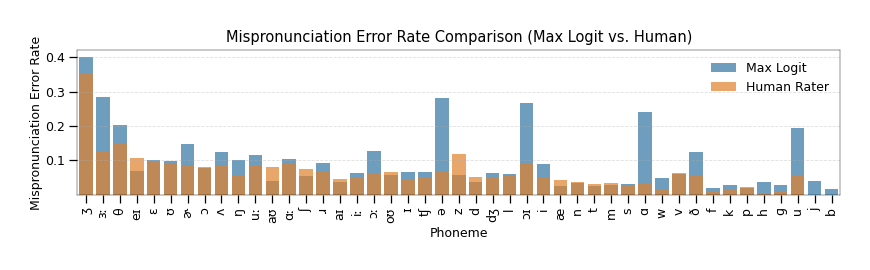
\includegraphics[width=0.8\textwidth]{comparison_error_rates_max_logit_vs_human_rater_small.png}
    \vspace{-0.6cm}
    \caption{Comparison of mispronunciation error rates by phoneme (Max Logit vs. human rater) in the SpeechOcean762 dataset. Blue bars show $\text{GOP}_{\text{MaxLogit}}$-predicted error rates, while red bars indicate human-rated phoneme accuracy.}
    \label{fig:maxlogit_vs_human}
\end{figure*}


To better interpret the performance results, Figure \ref{fig:gop_violin} visualizes the distribution of correctly pronounced and mispronounced phonemes across both datasets. GOP\textsubscript{DNN} shows a wide distribution overlap between correct and mispronounced phonemes in both cases (both graphs of Figure \ref{fig:gop_violin}), with close means and high variance, making it less effective for error distinction.
%
In contrast, GOP\textsubscript{MaxLogit} achieves  better separation, especially in MPC (first graph of Figure \ref{fig:gop_violin}), though overlap increases in SpeechOcean762 (second graph of Figure \ref{fig:gop_violin}), leading to higher variability. 
%
The best-performing score in MPC, GOP\textsubscript{Margin}, effectively classifies children's speech (first graph of Figure \ref{fig:gop_violin}), but struggles with greater distribution overlap in SpeechOcean762 (second graph of Figure \ref{fig:gop_violin}).
%
GOP\textsubscript{VarLogit} shows high variability and significant overlap in both cases, making it unreliable. 
%
GOP\textsubscript{Combined} balances probability- and logit-based approaches across both datasets, reducing overlap compared to GOP\textsubscript{DNN}. It presents a trade-off between classification accuracy from posterior probabilities and human correlation from logit-based scores. While we incorporated  GOP\textsubscript{Margin} in GOP\textsubscript{Combined}, GOP\textsubscript{MaxLogit} could also be considered, leaving the optimal choice undecided.



\begin{comment}
    

\begin{figure*}[bt!]
    \centering
    \subfloat[GOP score distribution - MPC Dataset]{%
        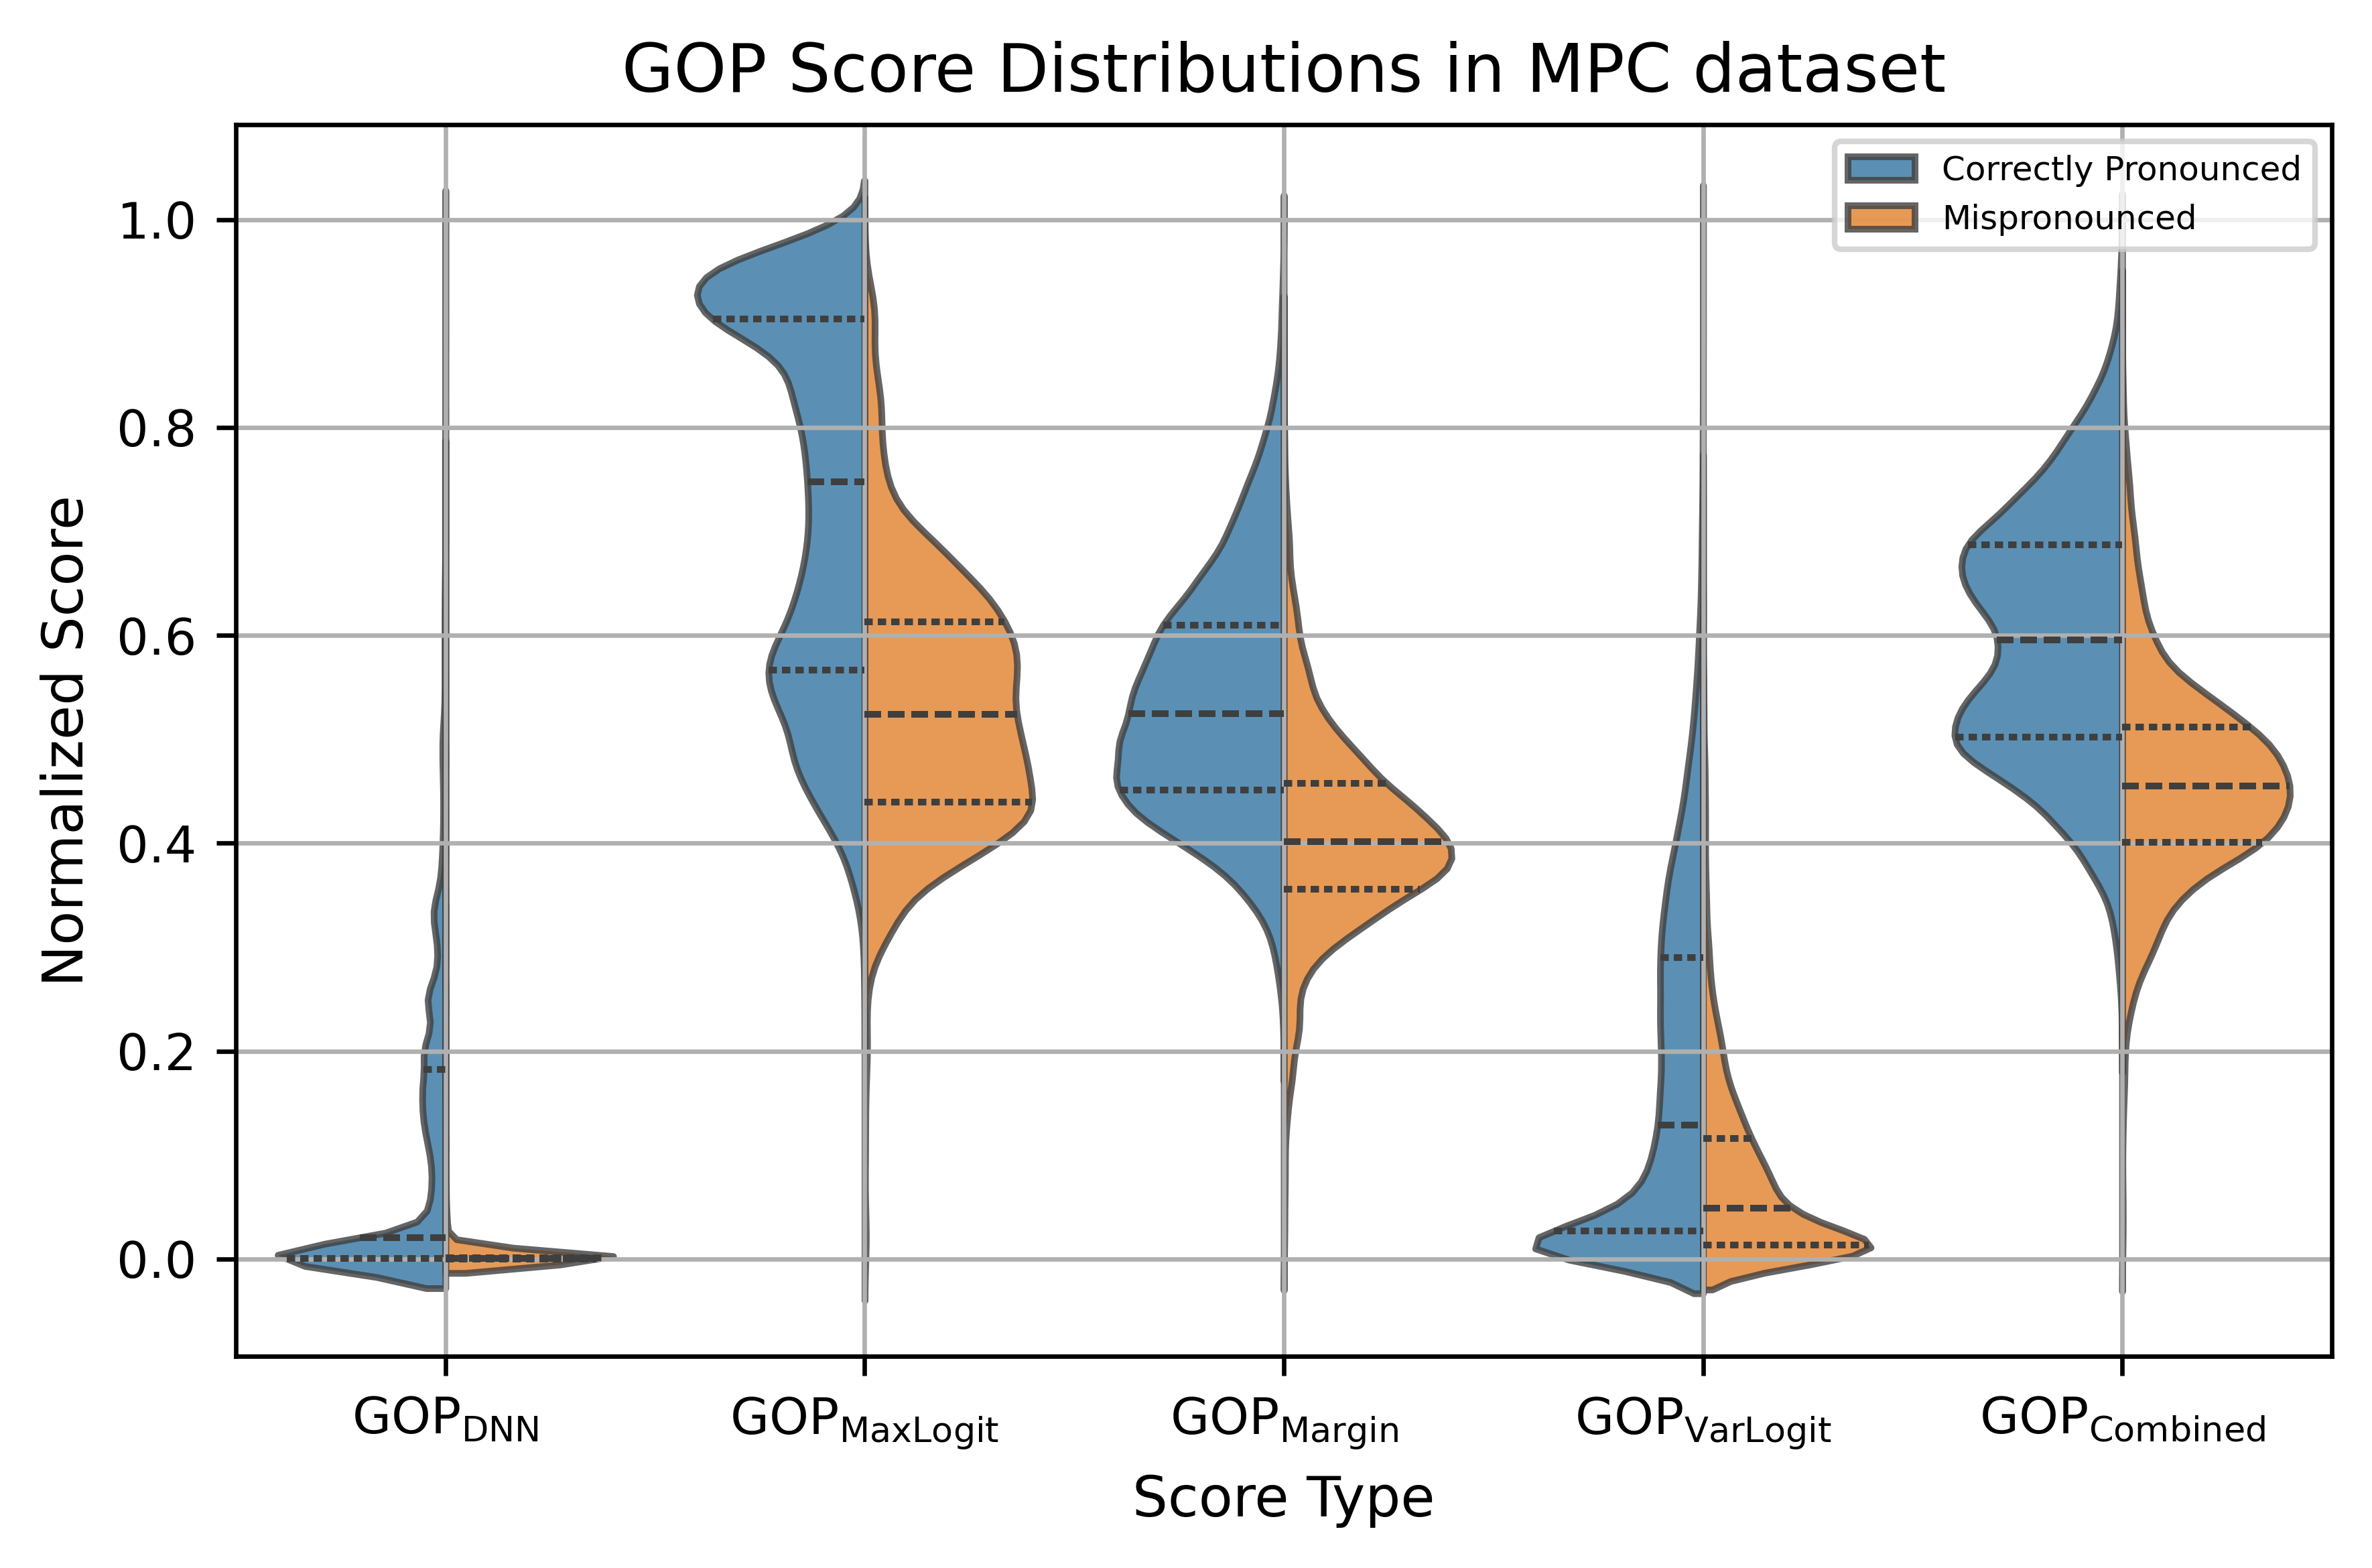
\includegraphics[width=0.4\textwidth]{MPC_VIOLIN_PLOT.png}%
        \label{fig:gop_violin1}%
    } \hfill
    \subfloat[GOP score distribution - Speechocean762 Dataset]{%
        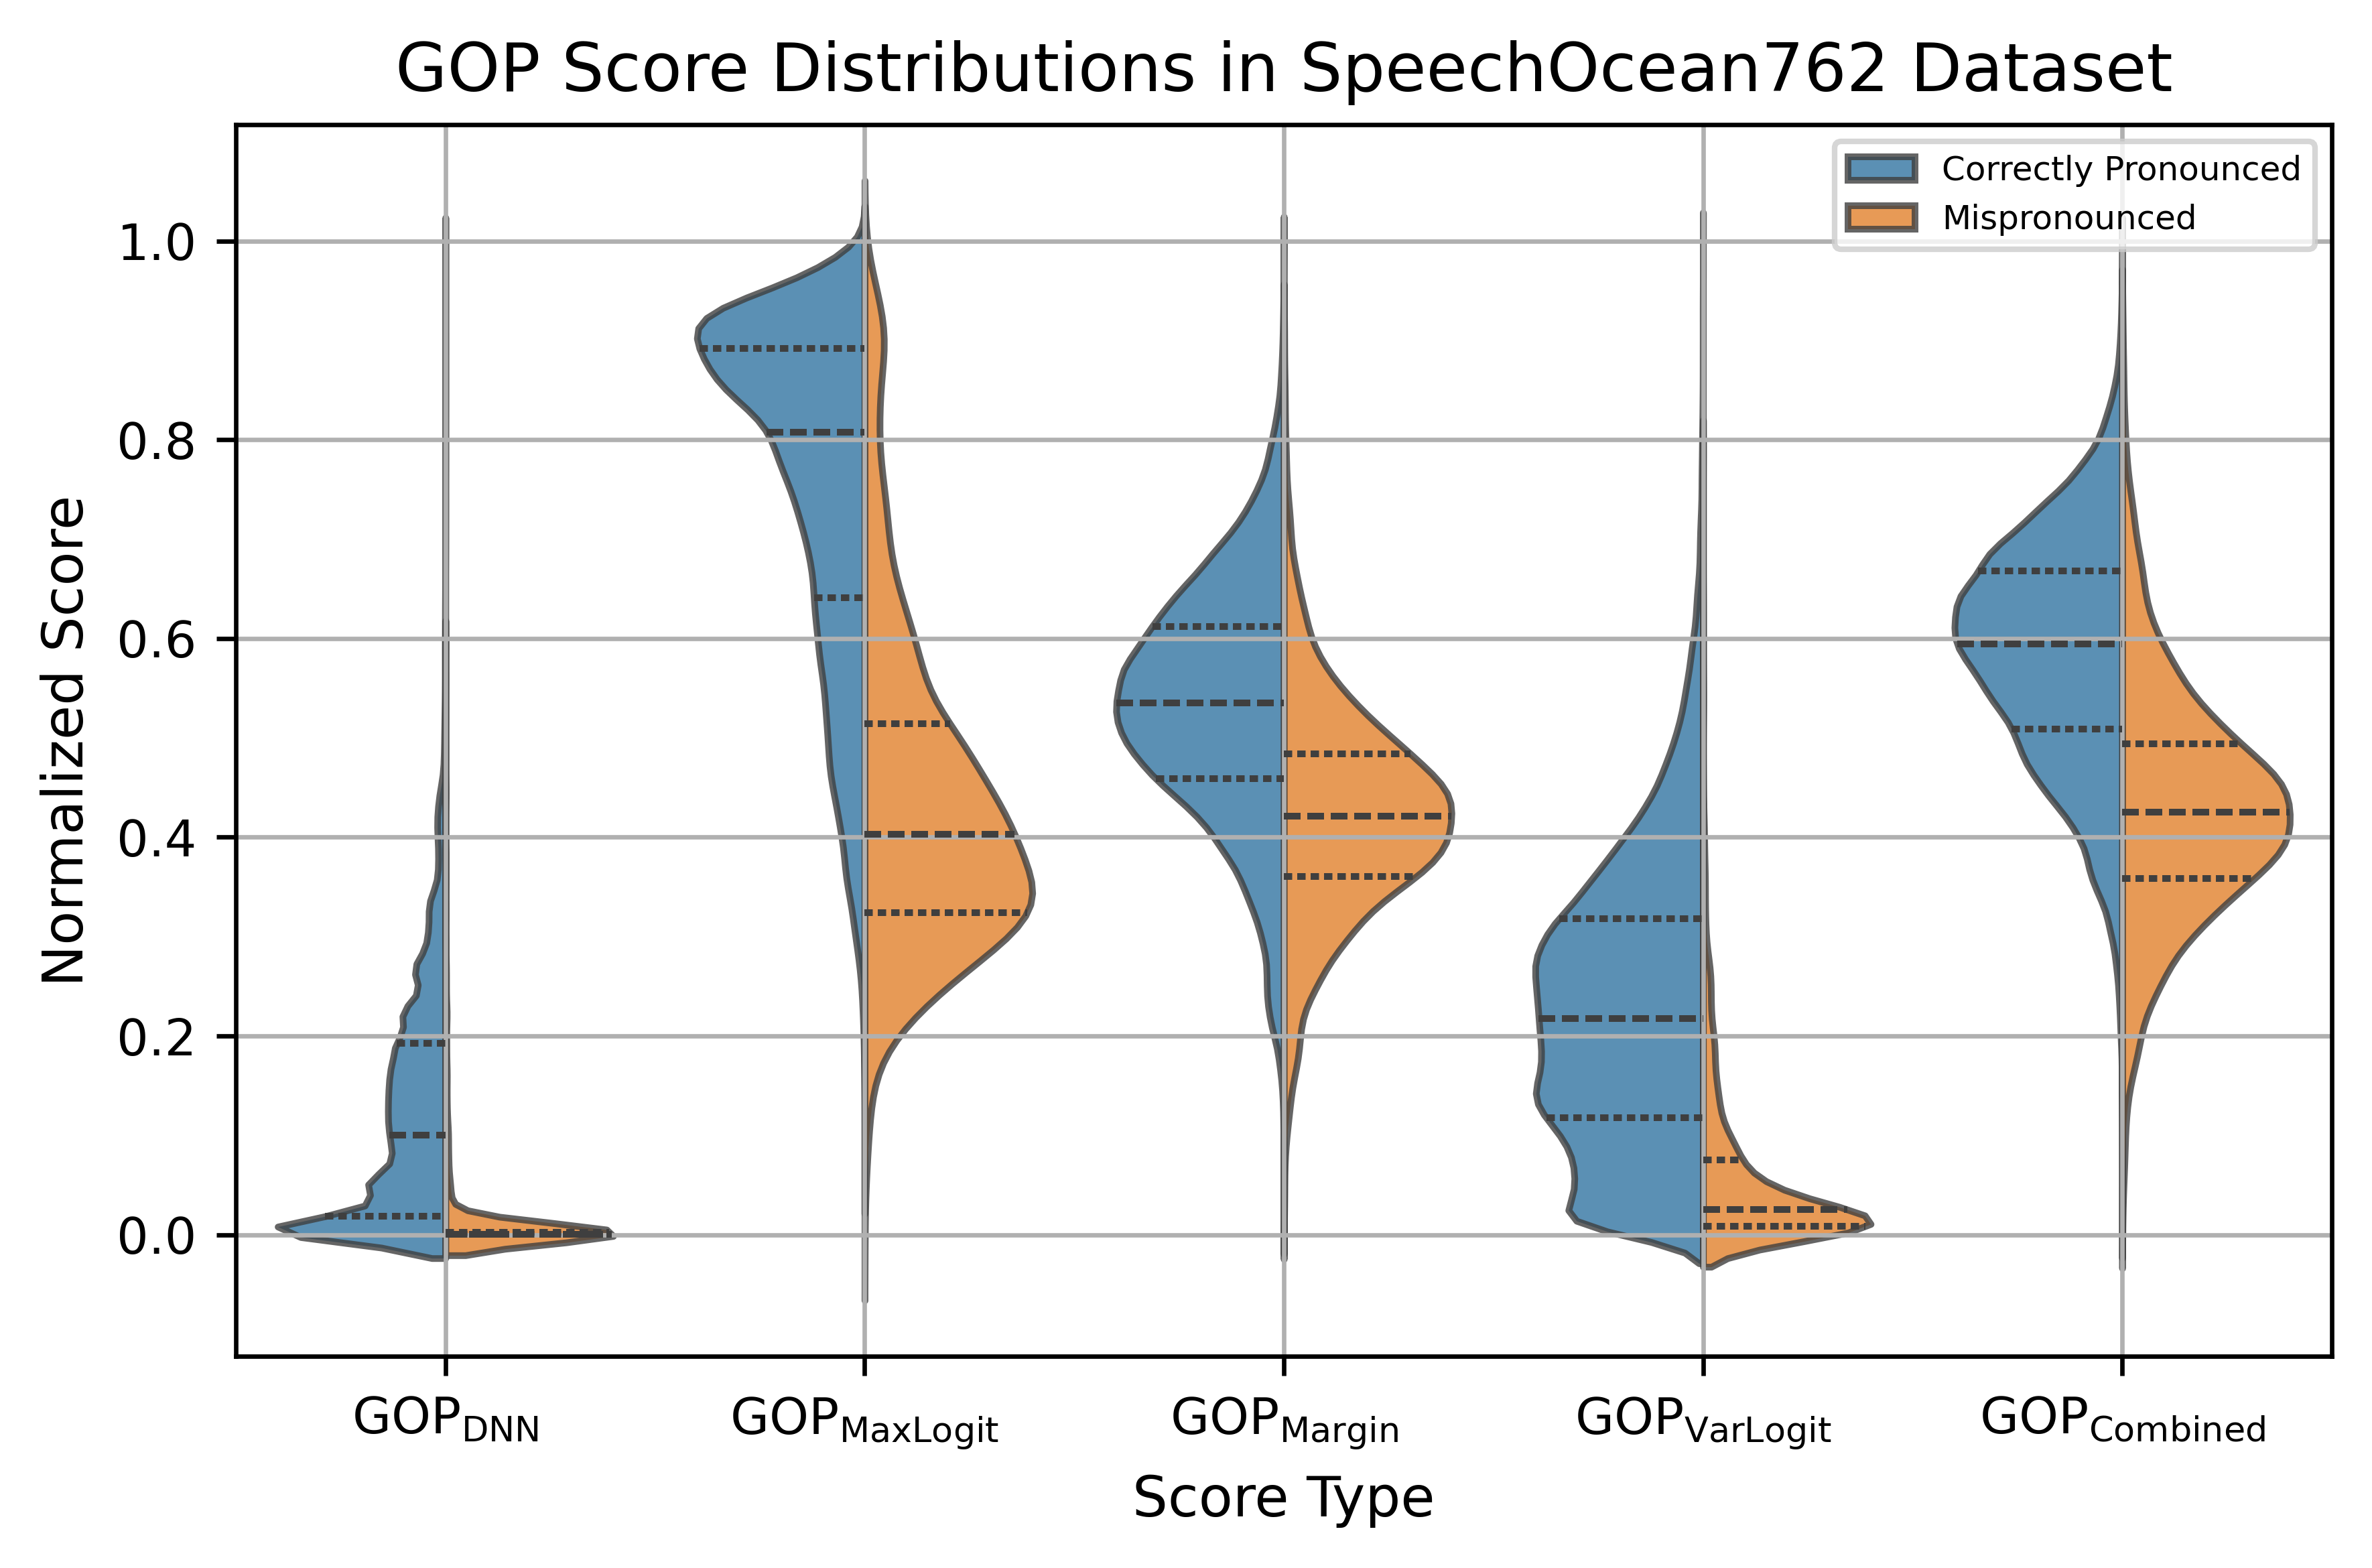
\includegraphics[width=0.4\textwidth]{speechocean_VIOLIN_PLOT.png}%
        \label{fig:gop_violin2}%
    }
    \vspace{-0.3cm}
    \caption{Comparison of GOP score distributions across MPC and Speechocean762 datasets.}
    \label{fig:gop_comparison}
\end{figure*}
\end{comment}


\begin{figure}[ht!]
    \centering
    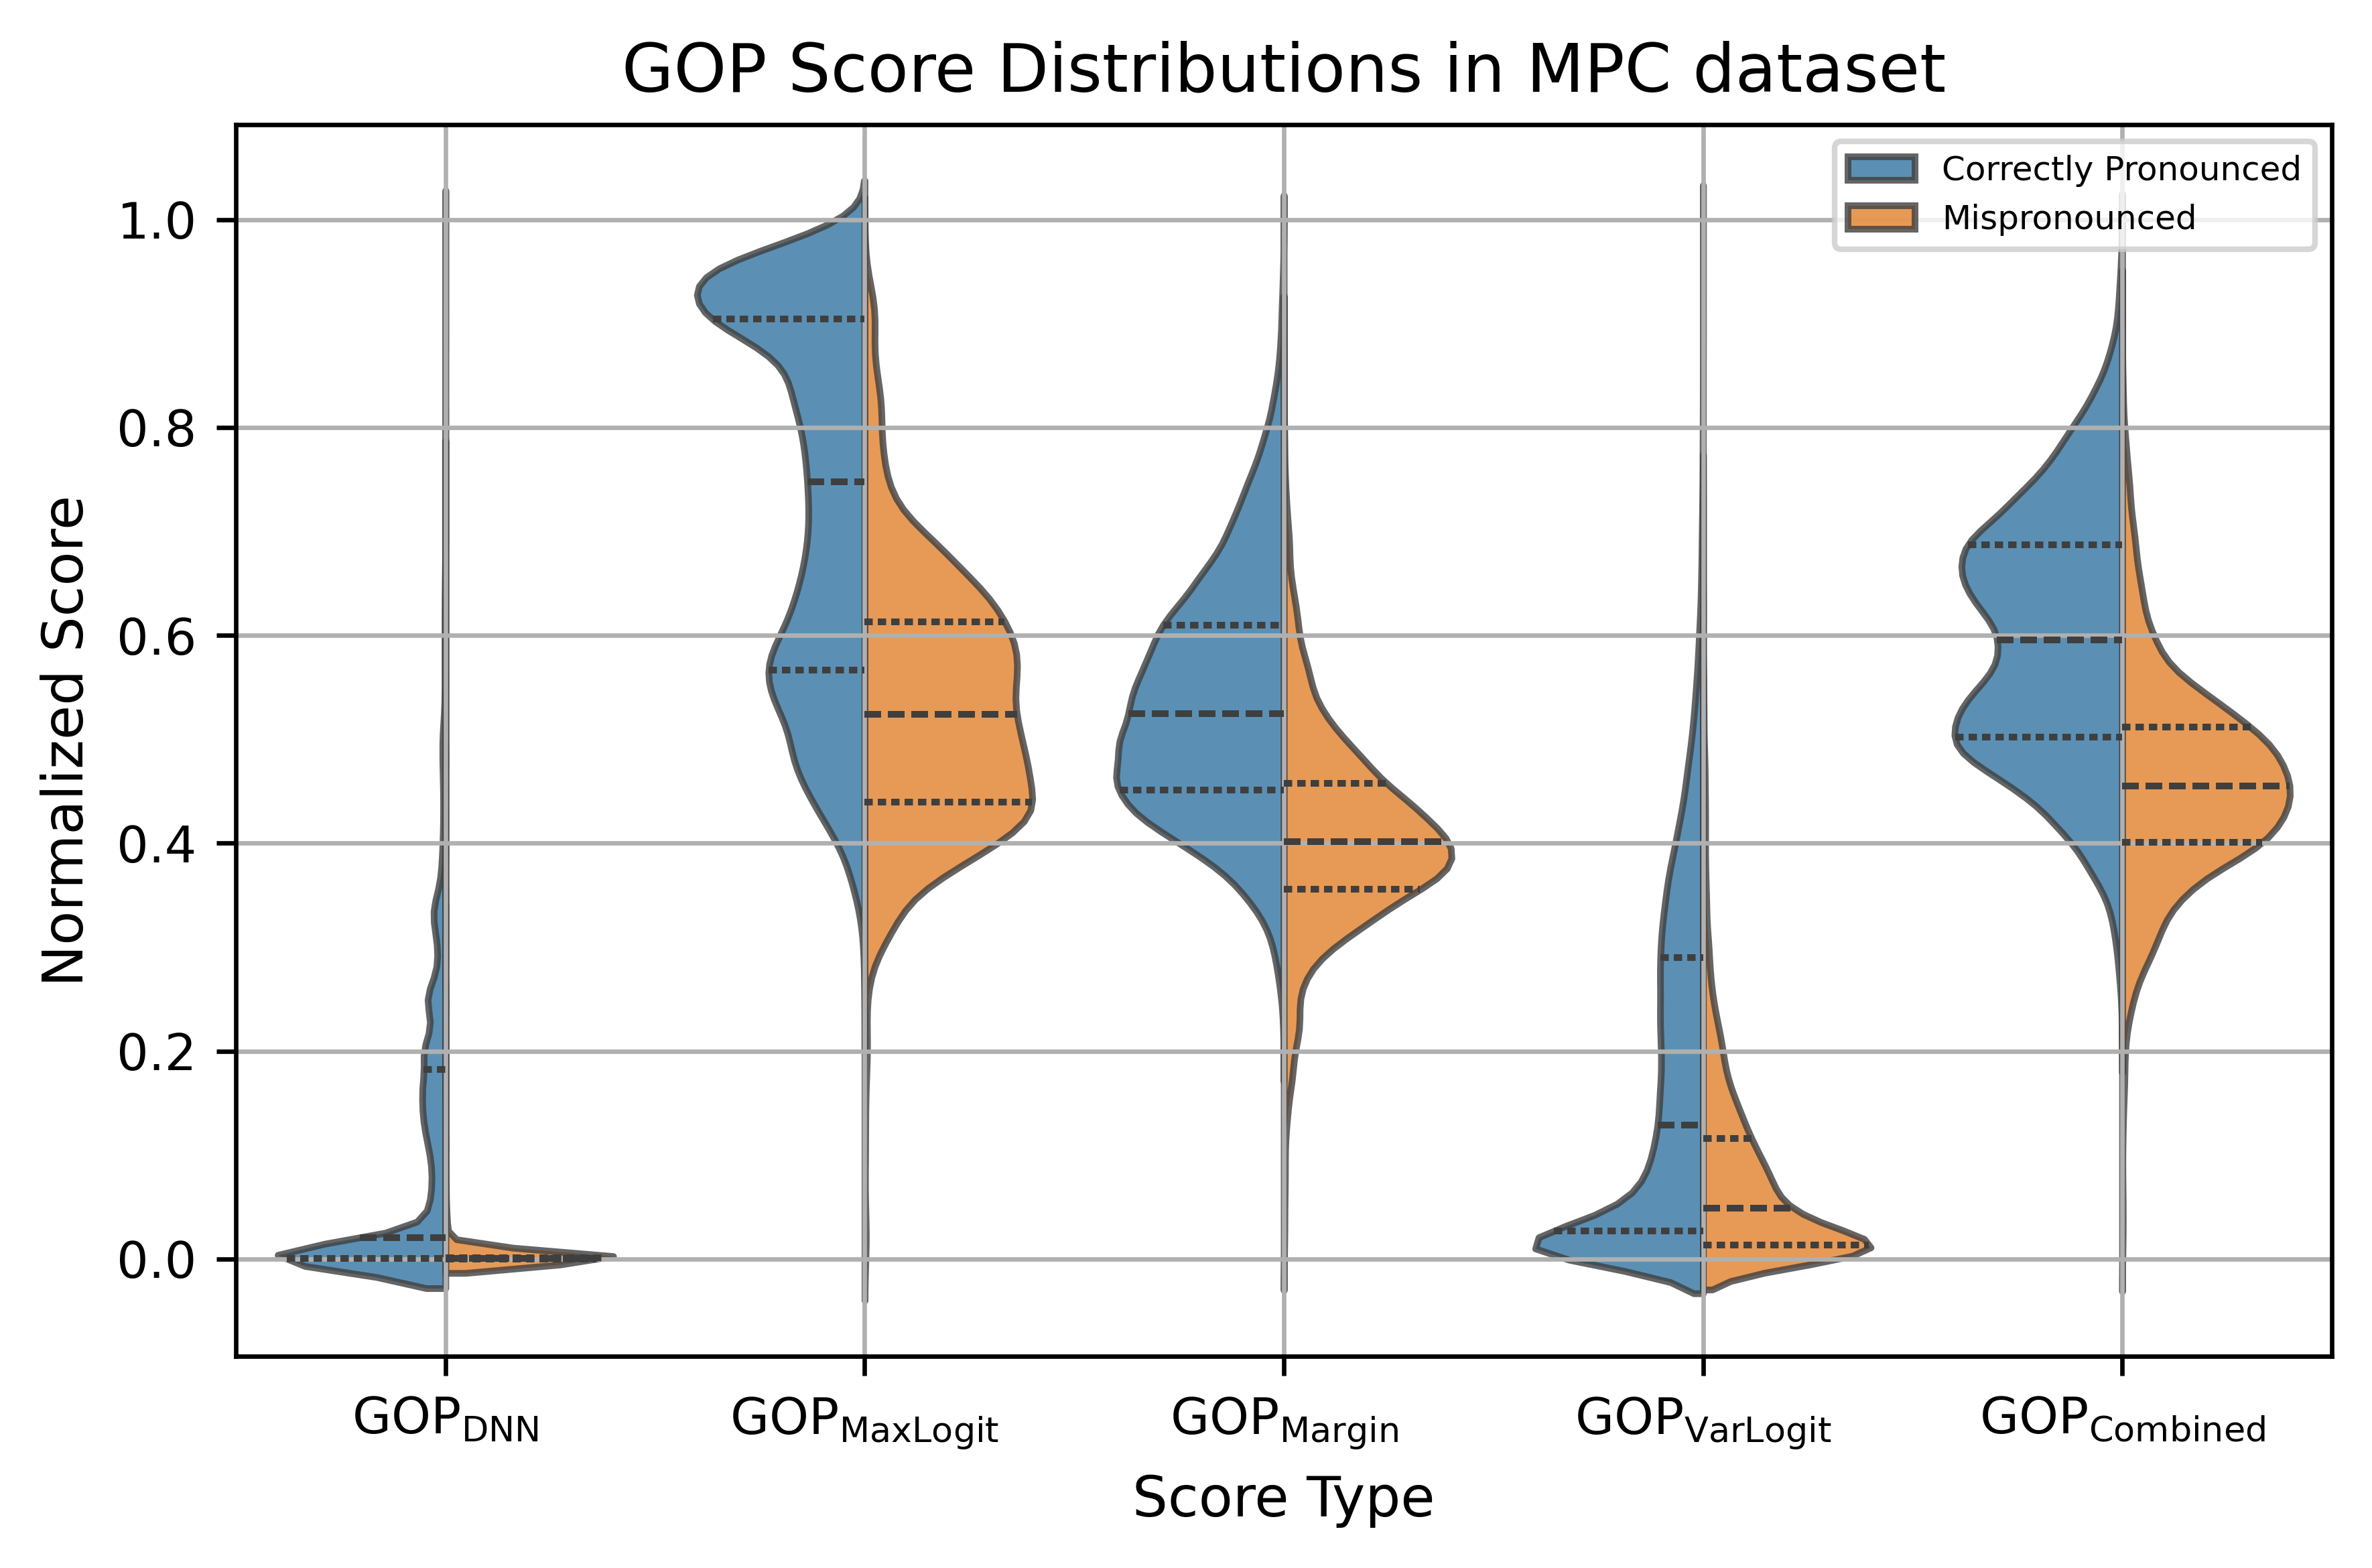
\includegraphics[width=0.35\textwidth]{MPC_VIOLIN_PLOT.png} %
    %%\caption{GOP score distribution - MPC dataset}
    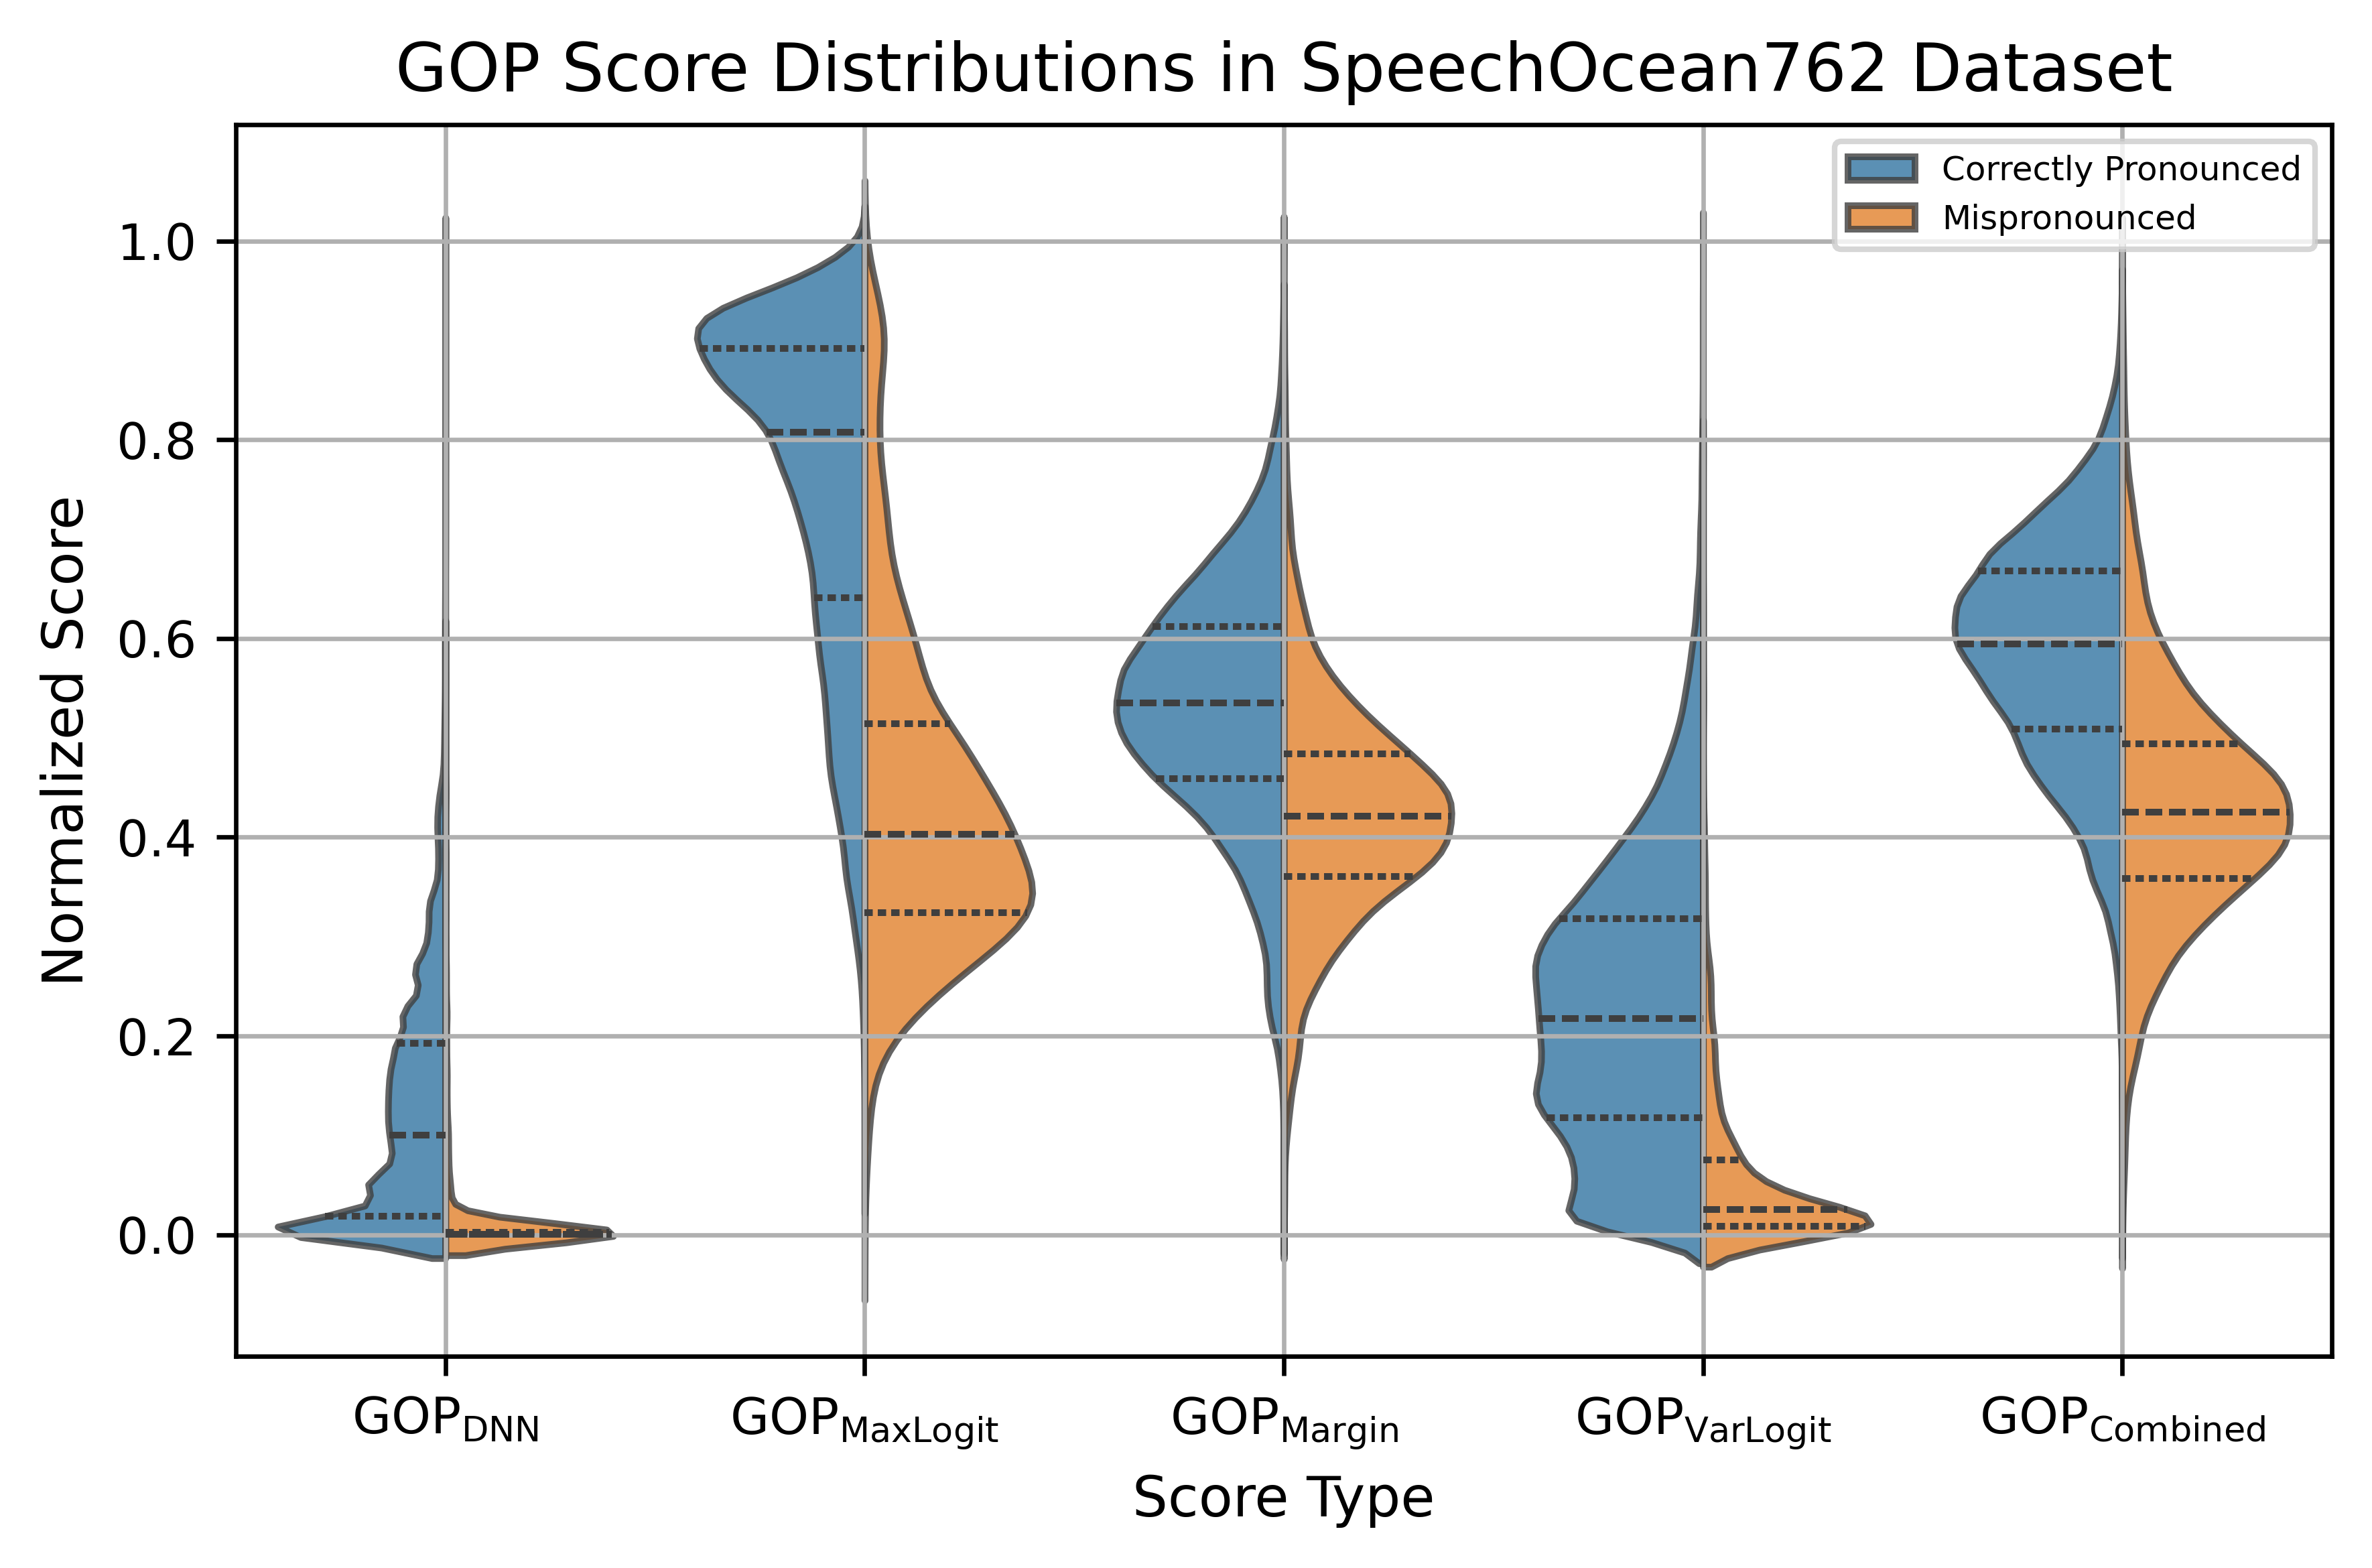
\includegraphics[width=0.35\textwidth]{speechocean_VIOLIN_PLOT.png}
    \vspace{-0.3cm}
   %% \caption{GOP score distribution - Speechocean762 dataset}
    
        \caption{Comparison of GOP score distributions across MPC and Speechocean762 datasets.}
    \label{fig:gop_violin}
\end{figure}

Finally, to analyze the alignment between GOP-based mispronunciation detection and human-rated phoneme accuracy, we investigated whether the GOP scoring method with the highest correlation to human ratings, GOP\textsubscript{MaxLogit}, effectively identifies mispronounced phonemes. Figure \ref{fig:maxlogit_vs_human} compares phoneme-level mispronunciation error rates predicted by GOP\textsubscript{MaxLogit} with human annotator ratings from the SpeechOcean762 dataset. Discrepancies were further examined by computing the difference in mispronunciation rates between GOP\textsubscript{MaxLogit} predictions and human ratings, highlighting phonemes where the model was overconfident, underconfident, or well-aligned (Figure \ref{fig:maxlogit_vs_human}). 
%

Phonemes where the GOP\textsubscript{MaxLogit} overestimates mispronunciations (meaning the model assigns significantly higher mispronunciation rates than human raters) include (top 5): /\textipa{@}/, /\textipa{A}/, /\textipa{OI}/, /\textipa{3:}/, and /\textipa{u}/. These phonemes are frequently flagged as mispronounced by the model, despite human raters considering them correctly pronounced in most instances. This suggests that GOP\textsubscript{MaxLogit} is overly confident for these phonemes, possibly misinterpreting slight articulatory variations as errors. Conversely, phonemes where GOP\textsubscript{MaxLogit} \textit{under}estimates mispronunciations (bottom 5), meaning human raters perceive more errors than the model detects, include /\textipa{\ae}/, /\textipa{S}/, /\textipa{eI}/, /\textipa{aU}/, and /\textipa{z}/. Some phonemes exhibit strong agreement between GOP\textsubscript{MaxLogit} predictions and human-rated error rates, indicating well-aligned phoneme classification. These phonemes are /\textipa{b}/, /\textipa{tS}/, /\textipa{i:}/, /\textipa{dZ}/, and /\textipa{A:}/.





\section{Discussion and Conclusion}

In this work, we have analyzed differences in probability-based and logit-based GOP for pronunciation assessment across two datasets, MPC and SpeechOcean762. To answer our RQ, %%—do logit-based GOP scores enhance mispronunciation detection compared to traditional GOP scores derived from softmax-based posterior probabilities?—
our findings indicate that logit-based methods achieve a better classification performance than probability-based GOP; however, their effectiveness depends on the characteristics of the dataset.
%
GOP\textsubscript{DNN} consistently obtains high recall, but low precision, indicating its tendency to over-detect mispronunciations, as seen in its high overlap between correctly pronounced and mispronounced phonemes. In contrast, logit-based methods (GOP\textsubscript{MaxLogit}) demonstrate better phoneme separation (Fig. \ref{fig:gop_violin}).

A key insight is that GOP\textsubscript{MaxLogit} aligns best with human ratings, achieving the highest PCC scores (Table \ref{tab:mpc-table}), while GOP\textsubscript{DNN}, despite strong classification performance, does not correlate well with expert judgments (Table \ref{tab:speechocean-table}). This suggests that maximum logit values better capture pronunciation quality from a perceptual standpoint. GOP\textsubscript{VarLogit} shows high variability (Table \ref{tab:mpc-table} and \ref{tab:speechocean-table}), making it less reliable, while GOP\textsubscript{Combined} balances probability and logit-based information but still shows some overlap. 

To the best of our knowledge, the highest PCC score reported on the SpeechOcean762 dataset is 0.69 \cite{chao23_interspeech}. However, this was achieved using a multidimensional MDD model that calculates GOP scores while incorporating additional aspects of speech in the SpeechOcean762 dataset. In contrast, our approach focuses solely on logit-based GOP scoring, making direct comparisons with these other methodologies challenging. Future research should focus on reducing reliance on forced alignment, which can introduce errors due to acoustic variability in child and non-native speech, contributing to high recall but low precision. 

In conclusion, our logit-based methodology offers a model-agnostic framework for any CTC-based acoustic model using a threshold-based approach. However, results vary across datasets, with GOP\textsubscript{Margin} performing best on MPC and GOP\textsubscript{MaxLogit} on SpeechOcean762, underscoring the role of acoustic variability.

%Despite our logit-based methodology being independent of specific datasets and not requiring an external MDD model, it remains a model-agnostic approach. As a result, it can be implemented in any CTC-based phoneme recognition model.

%Additionally, exploring how the proposed approach scales to new datasets remains an important direction for future investigation.



%The results suggest that a robust pronunciation assessment model should integrate both probability and logit-based features, optimizing GOP\textsubscript{Combined} with phoneme-specific weighting or uncertainty modeling. Future work should explore adaptive GOP thresholds and deep-learning-based fusion techniques to enhance mispronunciation detection.


\section{Acknowledgements}
This publication is part of the project Responsible AI for Voice Diagnostics (RAIVD) with file number NGF.1607.22.013 of the research programme NGF AiNed Fellowship Grants which is financed by the Dutch Research Council (NWO).




\bibliographystyle{IEEEtran}
\bibliography{mybib}

\end{document}